\chapter{Sintesi delle attività svolte durante lo stage}
	\section{Metodologia agile}
		\subsection{Pianificazione di iterazioni in modo adattivo}
			Durante lo svolgimento dello stage mi sono fortemente adattato al modo di lavorare tipicamente utilizzato in azienda.
			PastBook, infatti, utilizza una metodologia \emph{agile} per organizzare l'intero team e, in particolare, il gruppo di coloro
			che sono dedicati alla produzione del software. Questo approccio è particolarmente adatto all'azienda a causa delle sue
			ridotte dimensioni.\\
			La prima cosa che ho notato nel modo di lavorare dei miei colleghi è stato il fatto che essi inizino a svolgere le loro
			attività senza avere ben chiari tutti i requisiti che il prodotto dovrebbe soddisfare entro la fine del progetto.
			Essi, in particolare, fanno una pianificazione molto generica all'inizio di ciascun mese, concentrandosi più sugli
			obiettivi che dovrebbero raggiungere e sui requisiti da soddisfare piuttosto che sulle attività da eseguire per poter
			adempiere ai loro compiti. Di settimana in settimana, poi, ogni gruppo di progetto pianifica nel dettaglio tutto il lavoro
			che si dovrebbe svolgere. I progetti aziendali, dunque, procedono in modo adattivo piuttosto predittivo: il team preferisce
			adattare il modo di lavorare ai risultati ottenuti piuttosto che prevedere a priori ogni singola eventualità nel dettaglio.\\
			Per quanto mi riguarda, ho innanzitutto accordato con i mio tutor quali sarebbero stati gli obiettivi e i requisiti minimi
			da raggiungere durante i due mesi di stage. In seguito ho pianificato con cadenza settimanale i singoli task che avrei
			dovuto svolgere: ho cercato di rendere più granulare possibile ogi singolo comèito, in modo tale che non richiedesse più di
			mezz'ora per essere portato a termine. Una volta terminata l'iterazione ho analizzato i risultati raggiunti per capire se
			fossero sopraggiunte nuove difficoltà e quale sarebbe stato il modo migliore di aggiornare i requisiti.
		\subsection{Coinvolgimento diretto e continuo del cliente}
			Io e il team di sviluppo di cui facevo parte abbiamo coinvolto in modo continuo i clienti — che nel nostro caso
			corrispondevano al CTO e al dirigente — durante l'esecuzione di tutte le nostre attività. Essi hanno fornito feedback utili
			per capire pregi e difetti del prodotto: questo mi ha permesso di adattare il mio lavoro alle richieste dei clienti oltre che
			alle difficoltà incontrate.\\
			Con cadenza settimanale ho partecipato a brevi riunioni con il mio gruppo di lavoro e i clienti stessi. Durante questi
			meeting abbiamo discusso apertamente sullo stato di avanzamento del prodotto. Abbiamo inoltre evidenziato problemi che
			hanno rallentato lo sviluppo e che si sono rivelati essere più ardui del previsto: in questi casi abbiamo concordato delle
			modifiche ai requisiti richiesti. Eventuali nuove idee sono state vagliate in base al loro costo.
		\subsection{Consegne frequenti}
			Una mia costante preoccupazione durante l'intera durata dello stage è stata quella di effettuare numerosi rilasci di versioni
			intermedie del software prodotto. Questa prototipazione frequente è stata richiesta esplicitamente dal dirigente aziendale:
			egli intendeva testare costantemente le nuove funzionalità aggiunte di volta in volta.\\
			In particolare, quando ho cominciato lo sviluppo di My Year Photo Book ero tenuto a consegnare una versione funzionante
			dell'applicazione al termine di ogni giornata, salvo rare eccezioni. Effettuare rilasci frequenti di prototipi mi ha permesso
			di godere di alcuni vantaggi:
			\begin{itemize}
				\item Nel caso di eccessive difficoltà riscontrate durante lo sviluppo avevo sempre a disposizione una o più basi
				solide dalle quali sarei potuto ripartire. L'aggiunta di nuove caratteristiche non stravolgeva l'intero funzionamento
				dell'applicazione.
				\item Ero costretto a prestare la massima attenzione a non introdurre errori. La loro eventuale correzione aveva
				priorità assoluta poichè senza essa non avrei potuto ottenere un prototipo funzionante. Di conseguenza, l'attività di
				mantenimento dell'applicazione non è stata particolarmente impegnativa.
				\item Ho ricevuto numerosi feedback dai clienti che hanno avuto la possibilità di provare l'applicazione. Questi
				hanno in larga parte aiutato — e in parte sostituito — le mie attività di verifica e collaudo.
			 \end{itemize}
			 Lo svantaggio introdotto da questo approccio ha riguardato perlopiù la lentezza alla quale ero costretto a procedere.
		\subsection{Pair programming}
			Una delle tecniche più utilizzate in azienda è il \emph{pair programming}. Essa prevede che due programmatori lavorino
			ad una stessa postazione di lavoro: uno dei due scrive il codice ed ha l'obiettivo principale di realizzare una soluzione
			funzionante del problema in considerazione, l'altro svolge un ruolo di revisione simultanea del codice e gli è lasciato il
			compito di segnalare errori o proporre strategie alternative di soluzione.\\
			Ho partecipato a molte sessioni di pair programming, sia in qualità di programmatore che di osservatore, principalmente con
			il mio tutor. Ho sfruttato questa tecnica soprattutto nei momenti di difficoltà o comunque quando non era ben chiaro al
			gruppo di lavoro quale fosse la miglior strategia da perseguire. Il pair programming, in particolare, si è rivelato utile o
			addirittura indispensabile in due tipi di situazione:
			\begin{itemize}
				\item Tale tecnica mi ha aiutato durante le fasi iniziali dello sviluppo dei nuovi componenti. In azienda, infatti,
				non è previsto un vero e proprio momento in cui si progetta l'architettura del software e questi momenti di
				confronto con un programmatore più esperto mi hanno aiutato a individuare quali fossero le soluzioni più opportune
				da applicare ai vari casi.
				\item Questa tecnica è stata inoltre indispensabile durante la risoluzione di problemi particolarmente ardui alla
				quale partecipava anche il mio tutor. Infatti, non essendo previsa l'attività di stesura della documentazione del
				software, era difficile per una persona che non avesse mai programmato direttamente comprendere a fondo tutto il
				codice scritto da me. In questi casi ho dunque agito da supervisore, controllando che eventuali modifiche apportate
				non stravolgessero il funzionamento dell'applicazione e spiegando le ragioni per le quali avevo agito in un
				determinato modo piuttosto che in un altro.
			\end{itemize}
	\section{Attività preparatorie e di accompagnamento}
		\subsection{Configurazione dell'ambiente di lavoro}
			\subsubsection{Configurazione delle macchine virtuali}
				I primi giorni della mia esperienza di stage sono stati dedicati all'installazione e alla configurazione
				dell'ambiente con il quale avrei lavorato per i rimanenti due mesi. Quest'attività è stata costantemente
				supervisionata dal CTO di PastBook, che si è accertato che tutti gli strumenti necessari funzionassero in modo
				corretto.\\
				Ho cominciato con l'installazione della sandbox tramite la quale avrei potuto eseguire il collaudo dei miei prodotti
				senza dover interfacciarmi direttamente con i server aziendali. La configurazione di questo strumento è stata
				abbastanza agevole in quanto in azienda era disponibile una guida realizzata dal CTO che illustrava tutti i passi
				necessari. Ho contribuito al miglioramento della guida nei passaggi non sufficientemente chiari.
			\subsubsection{Installazione di Titanium e delle relative dipendenze}
				L'installazione dei vari componenti dell'ambiente di sviluppo Titanium e delle relative dipendenze è risultato
				essere molto semplice: Appcelerator, infatti, mette a disposizione eseguibili che si occupano in modo automatico
				della configurazione dei vari prodotti. Anche quando ho dovuto aggiornare la piattaforma durante la quinta settimana
				di stage (per poter supportare l'ultima versione di iOS) non ho riscontrato particolari problemi.\\
				Ciò che ha richiesto tempo, invece, è stata un'accurata analisi dei vari strumenti a disposizione degli sviluppatori,
				per capire quali di essi avrebbero potuto risultare utili ai miei scopi.\\
				Il primo strumento che ho studiato e analizzato è stato Appcelerator Studio, l'IDE gratuito messo a disposizione dai
				creatori di Titanium.
				\begin{center}
					\begin{tabular}[H]{| p{0.43\textwidth} | p{0.43\textwidth} |}
						\hline
						\emph{Pregi} di Appcelerator Studio &
						\emph{Difetti} di Appcelerator Studio\\
						\hline\hline
						È uno strumento sufficientemente semplice da essere utilizzato anche da sviluppatori alle prime armi.
						Allo stesso tempo esso mette a disposizione numerose funzionalità avanzate, dedicate a coloro che
						esigono strumenti complessi di analisi, debugging e test. &
						È estremamente lento nell'eseguire qualsiasi tipo di operazione, dalla più semplice alla più
						complessa. Questo accade anche su macchine recenti.\\
						\hline
						Fornisce metodi semplici ed efficaci per installare moduli aggiuntivi, evitando in questo modo allo
						sviluppatore di dover mettere mano ai file di configurazione stessi. Inoltre, permette la gestione
						automatica delle varie versioni delle API messe a disposizione dagli SDK di Android e iOS. &
						Un bug mai risolto fa in modo che l'utilizzo della RAM a disposizione sia inaccettabile. In
						particolare, ogni volta che un programmatore compila il codice viene creato un processo Node.js che
						non viene più chiuso: questo fa in modo che le risorse a disposizione dell'utente diventino sempre
						meno e che l'intero sistema rallenti nettamente con l'uso continuato.\\
						\hline
					\end{tabular}
				\end{center}
				Non ho tardato a realizzare come tale software fosse inadatto ad un utilizzo intensivo e giornaliero: esso rallentava
				troppo qualsiasi operazione che dovevo svolgere. Aveva tuttavia il pregio di aiutarmi a gestire lo scaricamento,
				l'installazione e la configurazione degli SDK mobile (con relativi emulatori) e dei vari moduli a me necessari. Ho
				dunque optato per utilizzarlo solo in modo occasionale come strumento di supporto. Per utilizzare tutte le altre
				funzionalità ho deciso di far uso di Titanium CLI (l'interfaccia a linea di comando della piattaforma Appcelerator):
				questo prodotto, sebbene meno intuitivo, non appesantiva in modo considerevole il sistema e soprattutto utilizzava la
				RAM in modo efficace.\\
				Il secondo strumento della piattaforma Appcelerator che ho valutato è stato il framework MVC Alloy. La scelta, in
				questo caso, riguardava se utilizzare Titanium in modalità classica o sfruttando Alloy.
				\begin{center}
					\begin{tabular}[H]{| p{0.20\textwidth} | p{0.35\textwidth} | p{0.35\textwidth} |}
						\hline
						&
						Titanium \emph{Classic}&
						Titanium \emph{Alloy}\\
						\hline\hline
						Linguaggi utilizzati &
						Uso di Javascript per la realizzazione di qualsiasi funzionalità. &
						Uso di Javascript per lo sviluppo del controller e del modello ; uso di XML per la realizzazione
						della struttura della view; uso di TSS (linguaggio simile a CSS) per definire lo stile della view.\\
						\hline
						Compilazione &
						Il codice Javascript viene tradotto nel linguaggio richiesto dalla piattaforma mobile. Segue la
						produzione di un eseguibile. &
						Il codice viene interamente tradotto in Javascript (causando un piccolo overhead). In seguito la
						compilazione procede come nel caso di Titanium Classic.\\
						\hline
					\end{tabular}
				\end{center}
				Qui la scelta è	stata molto più semplice: il leggero aumento dei tempi di compilazione causato dall'uso di Alloy
				è in larga parte compensato dal fatto che lo sviluppo di applicazioni sia molto più intuitivo. Questa semplicità è
				dovuta soprattutto alla grande somiglianza con la programmazione web che fa uso di HTML, CSS e Javascript. Ho quindi
				deciso di sfruttare il framework Alloy per la realizzazione dei prodotti che mi sono stati assegnati.\\
				Un ultimo strumento che ho valutato è stato \emph{Appcelerator LiveView}. Si tratta di un componente aggiuntivo per
				Titanium che serve per verificare e testare i cambiamenti apportati al codice in tempo reale. Esso permette ai
				programmatori di perdere meno tempo per i test. Il classico metodo utilizzato per verificare la correttezza
				di una certa modifica apportata consiste nel compilare il codice, trasferire l'eseguibile su un emulatore mobile e
				infine lanciare l'applicazione manualmente.\\
				\begin{figure}[H]
	\centering
	\begin{tikzpicture}
		\draw[fill=azzurro] (0,0.1\textwidth) rectangle ++(0.22\textwidth,0.06\textwidth);
		\draw (0,0.1\textwidth) rectangle ++(0.22\textwidth,0.06\textwidth)
		node[pos=.5, text width=0.17\textwidth, align=center] {Avvio applicazione};
		\draw[fill=azzurro] (0.25\textwidth,0) rectangle ++(0.22\textwidth,0.06\textwidth);
		\draw (0.25\textwidth,0) rectangle ++(0.22\textwidth,0.06\textwidth)
		node[pos=.5, text width=0.17\textwidth, align=center] {Installazione su emulatore};
		\draw[fill=azzurro] (0.5\textwidth,0.1\textwidth) rectangle ++(0.22\textwidth,0.06\textwidth);
		\draw (0.5\textwidth,0.1\textwidth) rectangle ++(0.22\textwidth,0.06\textwidth)
		node[pos=.5, text width=0.17\textwidth, align=center] {Compilazione};
		\draw[fill=azzurro] (0.09\textwidth,0.25\textwidth) rectangle ++(0.22\textwidth,0.06\textwidth);
		\draw (0.09\textwidth,0.25\textwidth) rectangle ++(0.22\textwidth,0.06\textwidth)
		node[pos=.5, text width=0.17\textwidth, align=center] {Verifica modifiche};
		\draw[fill=azzurro] (0.41\textwidth,0.25\textwidth) rectangle ++(0.22\textwidth,0.06\textwidth);
		\draw (0.41\textwidth,0.25\textwidth) rectangle ++(0.22\textwidth,0.06\textwidth)
		node[pos=.5, text width=0.17\textwidth, align=center] {Codifica};
		\draw[->] (0.32\textwidth,0.28\textwidth) -- (0.40\textwidth,0.28\textwidth);
		\draw[->] (0.24\textwidth,0.03\textwidth) -- (0.11\textwidth,0.09\textwidth);
		\draw[->] (0.11\textwidth,0.17\textwidth) -- (0.20\textwidth,0.24\textwidth);
		\draw[->] (0.52\textwidth,0.24\textwidth) -- (0.61\textwidth,0.17\textwidth);
		\draw[->] (0.61\textwidth,0.09\textwidth) -- (0.48\textwidth,0.03\textwidth);
	\end{tikzpicture}
	\caption{Ciclo necessario per la verifica delle modifiche}
\end{figure}

				\noindent LiveView, tuttavia, permette di aumentare enormemente la velocità dell'intero processo (passando da alcuni
				minuti a pochi secondi di attesa). L'unico problema di tale strumento è il fatto che sia tutt'ora molto instabile e
				non del tutto affidabile: spesso restituiva errori incomprensibili o causava il crash dell'applicazione in seguito a
				qualche test ripetuto. Nonostante l'enorme comodità che avrebbe potuto rappresentare, ho preferito non utilizzarlo
				in modo costante a causa dell'insicurezza dei suoi risultati. LiveView, tuttavia, è risultato particolarmente utile
				e stabile durante il design dell'applicazione: durante questa attività era inaccettabile compilare il codice
				ogniqualvolta si cambiava in modo minimo un colore o si spostava di qualche millimetro un elemento di una schermata.
			\subsubsection{Scelta e configurazione degli emulatori di dispositivi mobile}
				Gli ultimi strumenti che ho dovuto installare e configurare sono stati gli emulatori dei dispositivi mobile, sia per
				Android che iOS. Essi erano necessari durante lo sviluppo in quanto permettevano di testare l'applicazione senza far
				uso di telefoni fisici.\\
				Per quanto riguarda lo sviluppo sul sistema operativo prodotto da Apple, la scelta è stata obbligata: infatti, gli
				unici emulatori disponibili sono quelli che fanno parte dell'SDK stesso. Invece, per Android esistono più
				emulatori sul mercato, ognuno con caratteristiche e funzionalità più o meno avanzate. I due software tra i quali mi
				sono ritrovato a scegliere sono:
				\begin{itemize}
					\item \emph{Android Emulator}
					\item \emph{Genymotion}
				\end{itemize}
				Il primo è l'emulatore ufficiale ed è contenuto direttamente all'interno dell'SDK fornito da Google. Fornisce un
				gran numero di opzioni, tuttavia è abbastanza lento nell'esecuzione anche se installato all'interno di macchine
				recenti: questo fa in modo che sorgano non poche difficoltà riguardanti il collaudo di effetti grafici complicati. Il
				secondo software, invece, altro non è che una macchina virtuale Android installata all'interno di VirtuaBox (con
				l'aggiunta di funzionalità quali la simulazione dei vari tipi di sensori): esso si distingue dal rivale
				principalmente per la sua maggiore reattività ai comandi provenienti dall'utente. Genymotion, inoltre, possiede una
				seconda caratteristica che lo rende appetibile: è possibile installare le applicazioni semplicemente trasinandole
				all'interno dell'emulatore, senza dunque dover utilizzare più volte la linea di comando. La mia scelta, dunque, è
				ricaduta sulla seconda opzione.\\
				Una volta scelto l'emulatore ho speso un po di tempo a configurarlo affinchè si interfacciasse in modo corretto con
				la sandbox installata in locale. Questa operazione non era mai stata fatta in azienda e di conseguenza ho deciso di
				redigere una breve guida a riguardo, per aiutare in questo compito i futuri sviluppatori aziendali.
		\subsection{Studio e preparazione personale}
			Durante la prima settimana di stage ho dedicato molto del mio tempo a studiare il dominio applicativo. La mia formazione ha
			riguardato innanzitutto gli strumenti messi a disposizione dall'azienda:
			\begin{itemize}
				\item Ho preso confidenza con le API aziendali, servendomi della documentazione fornita da PastBook. Ho utilizzato
				Postman\footnote{Estensione per Google Chrome che permette di creare, organizzare, documentare e testare vari tipi di chiamate HTTP}
 per effettuare alcuni semplici test che mi permettessero di capire in
				modo più approfondito il funzionamento di questi servizi REST.
				\item Ho imparato ad utilizzare i Service aziendali. Per fare questo mi sono servito di test ed esempi già
				esistenti, in quanto PastBook non disponeva della documentazione relativa a tali servizi. Per studiare il modo in cui
				erano organizzati, per capire il loro scopo e per dedurre la tipologia di input richiesti ho avuto accesso
				direttamente al codice sorgente. Anche in questo caso il software Postman si è rivelato essere molto utile.
				\item Ho studiato il modo in cui l'azienda crea un Photo Book in automatico. Per fare ciò ho principalmente
				osservato il flusso di operazioni eseguite all'interno dell'applicazione web.
			\end{itemize}
			Durante quest'attività sono stato in stretto contatto con il tutor: egli mi ha aiutato a risolvere dubbi e mi ha fornito
			utili indicazioni che mi hanno permesso di apprendere in modo più veloce ed efficace.\\
			In secondo luogo, mi sono sforzato di assimilare le tecnologie che mi era stato richiesto di utilizzare durante la mia
			esperienza di stage. In particolare, gli aspetti fondamentali della mia attività di studio sono stati tre:
			\begin{itemize}
				\item Ho studiato le Titanium API che sono più comunemente usate. Mi sono soffermato su tutte quelle che sarebbero
				potute essere interessanti ai fini del mio lavoro. Ho cercato inoltre di approfondire la programmazione event-driven
				che tali API richiedono.
				\item Ho familiarizzato con Titanium CLI, l'interfaccia a linea di comando che è alla base dell'IDE messo a
				disposizione da Appcelerator e che è necessaria per la realizzazione degli eseguibili nativi per le varie piattaforme
				mobili su cui intendevo sviluppare. Ho individuato quali erano le funzionalità e i comandi che mi sarebbero
				probabilmente serviti durante la realizzazione del progetto assegnatomi.
				\item Ho cominciato a produrre alcuni semplici esempi che facessero uso del framework Alloy. Ho presentato questi
				test al mio tutor in modo tale che potesse fornirmi suggerimenti sui metodi migliori per utilizzare tale strumento.
			\end{itemize}
	\section{Sviluppo di PastBook Mobile SDK}
		\subsection{Autenticazione a Facebook e Instagram}
			\subsubsection{Studio del dominio e analisi dei requisiti}
				PastBook Mobile SDK deve innanzitutto permettere la gestione automatica dell'autenticazione a Facebook e Instagram.
				In assenza di questo requisito, infatti, molte delle API e dei Service aziendali non possono essere correttamente
				utilizzati in quanto necessitano di un'autorizzazione da parte dell'utente all'interno dei due social network.
				Dunque, ho avviato lo sviluppo dell'SDK studiando e analizzando le metodologie che permettono agli utenti di
				autenticarsi per poi autorizzare PastBook al trattamento dei loro dati.\\
				I processi di autenticazione e autorizzazione utilizzati da Facebook e Instagram sono molto simili e possono essere
				riassunti in questo modo:
				\begin{enumerate}
					\item Viene eseguito un controllo per capire se l'utente è già autenticato oppure no. Questo lo si può capire
					utilizzando una variabile \emph{login status}, che può essere memorizzata localmente o ottenuta in altri
					modi.
					\begin{itemize}
						\item Se l'utente è già autenticato si procede con il secondo passaggio.
						\item Se l'utente non è autenticato allora gli vengono richieste le sue credenziali.
						\begin{itemize}
							\item Se l'utente inserisce credenziali valide allora la variabile login status è aggiornata
							e si procede con il secondo passaggio.
							\item Se l'utente inserisce credenziali erronee allora esso viene avvertito ed è invitato
							provare nuovamente.
							\item L'utente può rifiutarsi di fornire le proprie credenziali. In questo caso il processo
							di autenticazione termina con un errore.
						\end{itemize}
					\end{itemize}
					\item Viene eseguito un controllo per capire se l'utente ha già fornito tutti i permessi richiesti
					dall'applicazione. Questo lo si può capire utilizzando una variabile \emph{granted permissions}, che può
					essere memorizzata localmente o ottenuta in altri modi.
					\begin{itemize}
						\item Se l'utente ha fornito tutti i necessari permessi allora si può procedere con il terzo
						passaggio.
						\item Se l'utente non ha fornito tutti i necessari permessi allora gli viene richiesto di
						autorizzarli.
						\begin{itemize}
							\item L'utente può confermare la propria autorizzazione a tutti i privilegi richiesti
							dall'applicazione. La variabile granted permissions viene aggiornata. In questo caso si
							procede con il terzo passaggio.
							\item L'utente può confermare la propria autorizzazione a una parte dei privilegi richiesti
							dall'applicazione. La variabile granted permissions viene aggiornata. Anche in questo caso
							si procede con il terzo passaggio.
							\item L'utente può negare l'autorizzazione dell'applicazione. In questo caso il processo di
							autorizzazione termina con un errore.
						\end{itemize}
					\end{itemize}
					\item Il server Facebook o Instagram restituisce al client un \emph{access token} che garantisce ad esso un
					accesso temporaneo e sicuro alle API del social network.
				\end{enumerate}
				\begin{figure}[H]
	\centering
	\begin{tikzpicture}
		\draw[fill=azzurro] (0,0.07\textwidth) rectangle ++(0.20\textwidth,0.12\textwidth);
		\draw (0,0.07\textwidth) rectangle ++(0.20\textwidth,0.12\textwidth)
		node[pos=.5, text width=0.18\textwidth, align=center] {Controllo stato autenticazione};
		\draw[->] (0.21\textwidth,0.13\textwidth) -- (0.25\textwidth,0.13\textwidth);
		\draw (0.1\textwidth,0.20\textwidth) -- (0.1\textwidth,0.27\textwidth);
		\draw (0.1\textwidth,0.27\textwidth) -- (0.61\textwidth,0.27\textwidth);
		\draw[->] (0.61\textwidth,0.27\textwidth) -- (0.61\textwidth,0.20\textwidth);
		\draw[fill=azzurro] (0.26\textwidth,0.07\textwidth) rectangle ++(0.20\textwidth,0.12\textwidth);
		\draw (0.26\textwidth,0.07\textwidth) rectangle ++(0.20\textwidth,0.12\textwidth)
		node[pos=.5, text width=0.18\textwidth, align=center] {Autenticazione};
		\draw[->] (0.47\textwidth,0.13\textwidth) -- (0.51\textwidth,0.13\textwidth);
		\draw[fill=azzurro] (0.52\textwidth,0.07\textwidth) rectangle ++(0.20\textwidth,0.12\textwidth);
		\draw (0.52\textwidth,0.07\textwidth) rectangle ++(0.20\textwidth,0.12\textwidth)
		node[pos=.5, text width=0.18\textwidth, align=center] {Controllo stato autorizzazione};
		\draw[->] (0.73\textwidth,0.13\textwidth) -- (0.77\textwidth,0.13\textwidth);
		\draw[fill=azzurro] (0.78\textwidth,0.07\textwidth) rectangle ++(0.20\textwidth,0.12\textwidth);
		\draw (0.78\textwidth,0.07\textwidth) rectangle ++(0.20\textwidth,0.12\textwidth)
		node[pos=.5, text width=0.18\textwidth, align=center] {Autorizzazione};
		
		\draw[dashed] (0.49\textwidth,0.2\textwidth) -- (0.49\textwidth,0.13\textwidth);
		\draw (0.41\textwidth,0.2\textwidth) rectangle ++(0.16\textwidth,0.06\textwidth)
		node[pos=.5, text width=0.16\textwidth, align=center] {Credenziali corrette};
		
		\draw (0.39\textwidth,0.06\textwidth) -- (0.39\textwidth,0);
		\draw (0.39\textwidth,0) -- (0.43\textwidth,0);
		\draw[->] (0.43\textwidth,0) -- (0.43\textwidth,0.06\textwidth);
		\draw[dashed] (0.43\textwidth,0.03\textwidth) -- (0.47\textwidth,0.03\textwidth);
		\draw (0.47\textwidth,0) rectangle ++(0.16\textwidth,0.06\textwidth)
		node[pos=.5, text width=0.16\textwidth, align=center] {Credenziali errate};
		
		\draw (0.36\textwidth,0.06\textwidth) -- (0.36\textwidth,-0.07\textwidth);
		\draw[->] (0.36\textwidth,-0.07\textwidth) -- (0.38\textwidth,-0.07\textwidth);
		\draw (0.88\textwidth,0.06\textwidth) -- (0.88\textwidth,-0.07\textwidth);
		\draw[->] (0.88\textwidth,-0.07\textwidth) -- (0.6\textwidth,-0.07\textwidth);
		\draw[fill=azzurro] (0.39\textwidth,-0.13\textwidth) rectangle ++(0.20\textwidth,0.12\textwidth);
		\draw (0.39\textwidth,-0.13\textwidth) rectangle ++(0.20\textwidth,0.12\textwidth)
		node[pos=.5, text width=0.18\textwidth, align=center] {Errore};
		
		\draw[->] (0.63\textwidth,0.2\textwidth) -- (0.63\textwidth,0.32\textwidth);
		\draw (0.88\textwidth,0.2\textwidth) -- (0.88\textwidth,0.35\textwidth);
		\draw[->] (0.88\textwidth,0.35\textwidth) -- (0.73\textwidth,0.35\textwidth);
		
		\draw[dashed] (0.83\textwidth,0.39\textwidth) -- (0.83\textwidth,0.35\textwidth);
		\draw (0.75\textwidth,0.39\textwidth) rectangle ++(0.16\textwidth,0.06\textwidth)
		node[pos=.5, text width=0.16\textwidth, align=center] {Concessi uno o più permessi};
		
		\draw[fill=azzurro] (0.52\textwidth,0.33\textwidth) rectangle ++(0.20\textwidth,0.12\textwidth);
		\draw (0.52\textwidth,0.33\textwidth) rectangle ++(0.20\textwidth,0.12\textwidth)
		node[pos=.5, text width=0.18\textwidth, align=center] {Ottenimento token};
		
		\draw[dashed] (0.36\textwidth,-0.04\textwidth) -- (0.31\textwidth,-0.04\textwidth);
		\draw (0.15\textwidth,-0.11\textwidth) rectangle ++(0.16\textwidth,0.1\textwidth)
		node[pos=.5, text width=0.16\textwidth, align=center] {Mancato inserimento credenziali};
		
		\draw[dashed] (0.75\textwidth,0.2\textwidth) -- (0.75\textwidth,0.13\textwidth);
		\draw (0.67\textwidth,0.2\textwidth) rectangle ++(0.16\textwidth,0.1\textwidth)
		node[pos=.5, text width=0.16\textwidth, align=center] {Alcuni permessi mancanti};
		
		\draw[dashed] (0.49\textwidth,0.3\textwidth) -- (0.63\textwidth,0.3\textwidth);
		\draw (0.33\textwidth,0.28\textwidth) rectangle ++(0.16\textwidth,0.1\textwidth)
		node[pos=.5, text width=0.15\textwidth, align=center] {Applicazione già autorizzata};
		
		\draw[dashed] (0.75\textwidth,-0.04\textwidth) -- (0.75\textwidth,-0.07\textwidth);
		\draw (0.67\textwidth,-0.04\textwidth) rectangle ++(0.16\textwidth,0.1\textwidth)
		node[pos=.5, text width=0.16\textwidth, align=center] {Nessun permesso concesso};
		
		\draw[dashed] (0.23\textwidth,0.13\textwidth) -- (0.23\textwidth,0.06\textwidth);
		\draw (0.15\textwidth,0) rectangle ++(0.16\textwidth,0.06\textwidth)
		node[pos=.5, text width=0.16\textwidth, align=center] {Utente non autenticato};
		
		\draw[dashed] (0.2\textwidth,0.27\textwidth) -- (0.2\textwidth,0.32\textwidth);
		\draw (0.12\textwidth,0.32\textwidth) rectangle ++(0.16\textwidth,0.06\textwidth)
		node[pos=.5, text width=0.16\textwidth, align=center] {Utente autenticato};
	\end{tikzpicture}
	\caption{Ottenimento token da Facebook o Instagram per l'autorizzazione dell'applicazione}
\end{figure}

				\noindent Ho subito capito che — per poter essere veramente robusto — l'SDK avrebbe dovuto saper gestire numerosi
				casi particolari. I più critici sono i seguenti:
				\begin{itemize}
					\item L'applicazione richiede l'autorizzazione per poter ottenere alcuni permessi da parte dell'utente
					(immagini e principali dati personali). In assenza di uno di questi elementi, le API e i Service PastBook non
					sono in grado di funzionare. Tuttavia, il processo di autenticazione e autorizzazione va a buon fine anche
					nel caso in cui l'utente non fornisca tutti i privilegi richiesti. L'SDK, dunque, deve preoccuparsi della
					gestione di questo caso, avvisando in modo consono l'applicazione affinchè essa decida cosa debba essere
					fatto.
					\item Molto spesso può accadere che un utente provi un'applicazione solo per curiosità. Tipicamente egli
					garantisce tutti i permessi necessari. In seguito egli può rimuovere uno o più privilegi dell'applicazione
					(questo può essere fatto all'interno del proprio profilo Facebook o Instagram). Nel peggiore dei casi
					l'utente può anche decidere di rimuovere completamente l'applicazione dal proprio profilo. 
					Tuttavia, l'SDK PastBook non ha modo di sapere quanto è successo e, se la variabile granted permissions è
					memorizzata localmente, esso sarà convinto che l'utente abbia correttamente fornito tutti i permessi
					necessari. Ciò provoca un errore all'interno dell'applicazione qualora l'utente tenti di utilizzarla
					nuovamente. È dunque necessario un meccanismo che eviti questi errori.
				\end{itemize}
			\subsubsection{Implementazione dell'autenticazione a Facebook tramite un modulo Titanium}
				Invece di implementare da zero l'autenticazione a Facebook ho deciso di utilizzare il modulo ufficiale per Titanium
				che Appcelerator mette a disposizione degli sviluppatori. Non ho preso la decisione opposta in quanto la cosa
				avrebbe richiesto una gestione coerente delle variabili granted permissions e login status: le complicazioni
				sarebbero probabilmente state eccessive. Inoltre, il modulo in questione mette a disposizione un'interfaccia
				molto semplice da utilizzare e permette l'autenticazione usando l'eventuale applicazione Facebook installata sul
				dispositivo mobile\\
				Grazie all'utilizzo di questo modulo sono stato in grado di gestire con poche righe di codice tutte le situazioni più
				comuni. In particolare, lo sviluppatore di applicazioni che utilizzi il PastBook Mobile SDK ha a disposizione
				l'interfaccia di una singola classe tramite la quale deve solo indicare che all'utente deve essere richiesta
				l'autenticazione a Facebook con conseguente autorizzazione dell'applicazione in questione. Il resto viene fatto
				dall'SDK. Tale componente lascia che il modulo Titanium si occupi della gestione delle credenziali dell'utente e
				della richiesta dei permessi necessari: il suo compito, piuttosto, è quello di nascondere allo sviluppatore di
				applicazioni la complessità riguardante la gestione dei casi particolari individuati durante l'attività di analisi
				dei requisiti. In particolare, l'SDK fa in modo che anche nei seguenti casi il comportamento del software prodotto
				sia corretto:
				\begin{itemize}
					\item Dopo aver utilizzato l'applicazione, l'utente rimuove uno o più permessi direttamente dalle
					impostazioni del suo profilo Facebook, per poi tentare di utilizzare nuovamente l'applicazione.
					\item L'utente tenta di utilizzare l'applicazione senza fornire tutti i permessi necessari.
				\end{itemize}
				Ho risolto il primo caso semplicemente aggiornando l'elenco dei permessi garantiti all'applicazione ogni volta che
				questa inizia ad utilizzare il PastBook Mobile SDK. In seguito ho controllato che tutti i privilegi di cui
				l'applicazione dovrebbe disporre siano contenuti all'interno dell'elenco ottenuto dai server di Facebook. Per quanto
				riguarda il secondo caso, invece, ho applicato un procedimento simile a quello descritto in precedenza. In
				particolare, in seguito a qualsiasi autorizzazione cerco di ottenere dai server Facebook i privilegi di cui
				l'applicazione dispone. Se questi sono corretti allora significa che l'autorizzazione è andata a buon fine,
				altrimenti deve essere gestita un'anomalia.\\
				Non sono invece riuscito a gestire in modo consono il caso in cui l'utente, dopo aver utilizzato l'applicazione, la
				rimuovesse completamente dal proprio profilo Facebook per poi tentare di utilizzarla nuovamente. Infatti, il modulo
				di Titanium non fornisce questa possibilità. Poichè per l'azienda questa cosa non era accettabile, in comune accordo
				con il mio tutor sono giunto a un compromesso che non era formalmente corretto ma che funzionava nella pratica. Nello
				specifico, ho sfruttato il fatto che in questo caso il modulo di Titanium restituiva un generico errore: tale
				malfunzionamento poteva essere generato da molti aspetti, tuttavia durante i numerosi test risultava accadere proprio
				il contrario (ovvero non è mai successo che venissero segnalati errori per altre ragioni). In presenza di un errore
				del modulo Facebook, dunque, davo per scontato che l'utente avesse rimosso l'autorizzazione all'applicazione dal
				proprio profilo e gestivo la situazione di conseguenza.\\
				Infine, ho optato per fornire sempre all'utilizzatore dell'SDK un feedback circa quanto accadesse durante il
				processo di autenticazione e autorizzazione: in questo modo egli può decidere comportamenti diversi per la propria
				applicazione, per esempio mostrando appropriati messaggi all'utente. Nel dettaglio, il feedback avverte lo
				sviluppatore di questi casi:
				\begin{itemize}
					\item l'utente non ha voluto inserire le proprie credenziali;
					\item l'utente non ha voluto autorizzare l'applicazione;
					\item l'utente ha autorizzato l'applicazione ma non ha fornito tutti i permessi necessari.
				\end{itemize}
				In definitiva, durante lo sviluppo di applicazioni si può utilizzare il componente dell'SDK per l'autenticazione e
				l'autorizzazione a Facebook nel seguente modo:
				\begin{lstlisting}
	...
	fbAuth = new facebookAuthentication();
	...
	fbAuth.authorize(function(e) {
		if (e.success) {
			var fbToken = fbAuth.getToken();
			// operazioni con il token restituito da Facebook
		}
		else if (e.cancelled) {
			// l'utente non ha voluto inserire le proprie credenziali
		}
		else {
			// gestione degli errori sulla base del contenuto di e.error
		}
	});
\end{lstlisting}

				L'utilizzo del modulo dedicato a Facebook realizzato da Appcelerator ha causato molti problemi durante
				l'implementazione dell'SDK, facendo perdere tempo prezioso. In particolare, il suo comportamento all'interno della
				piattaforma Android era completamente non coerente con quanto dichiarato nella documentazione ufficiale. I problemi
				riscontrati sono stati i seguenti:
				\begin{itemize}
					\item il \emph{login event} era sollevato quando il modulo era inizializzato oltre che in seguito
					all'effettiva autenticazione da parte dell'utente;
					\item la funzione per effettuare la disconnessione dal proprio account non aggiornava in modo corretto le
					variabili di stato, lasciando il sistema in una situazione inconsistente.
				\end{itemize}
				A causa di questi problemi ho dovuto implementare una versione apposita per Android del componente dedicato a
				Facebook che aggirasse questi difetti di base.
			\subsubsection{Implementazione dell'autenticazione a Instagram tramite API native}
				Ho eseguito un'approfondita ricerca sul web per trovare un modulo Titanium dedicato a Insagram simile a quello
				fornito per Facebook. Tuttavia, mi sono reso conto che tutti i software esistenti erano di qualità scadente o
				offrivano un'interfaccia grafica troppo basilare. Ho dunque optato per implementare personalmente l'autenticazione
				a questo social network, utilizzando le API messe a disposizione degli sviluppatori.\\
				Durante l'implementazione mi sono reso conto che fosse impossibile delegare all'eventuale applicazione Instagram
				installata sul dispositivo la responsabilità di gestire le credenziali e i vari permessi. Ho quindi scelto di
				incapsulare all'interno di una \emph{webview} il sistema di autenticazione e autorizzazione dedicato agli utenti che
				accedono al social network da browser. Questo modo di operare mi ha consentito di ottenere i seguenti vantaggi:
				\begin{itemize}
					\item \emph{velocità} nella realizzazione, in quanto gran parte del lavoro era già stata eseguita;
					\item \emph{sicurezza} del prodotto finale, perché relegata direttamente agli sviluppatori di Instagram;
					\item \emph{design} conforme a quello utilizzato dal social network stesso.
				\end{itemize}
				Sono anche riuscito a gestire i vari casi che possono avvenire durante il processo di autenticazione e autorizzazione
				e che avevo individuato durante la precedente attività di analisi. In particolare, mi è bastato effettuare il
				\emph{parsing} dell'url nelle varie situazioni per ottenere tutti i parametri di cui necessitavo.\\
				Per evitare allo sviluppatore il compito di integrare la webview all'interno del proprio prodotto e per ottenere allo
				stesso tempo un comportamento simile all'autenticazione tramite Facebook (che fa uso dell'applicazione esterna del
				social network), ho optato per fare in modo che l'SDK apra una nuova finestra all'interno della quale è inserita la
				webview. Al termine dell'autenticazione — o in caso di errori — tale finestra viene chiusa e il controllo del flusso
				torna nuovamente allo sviluppatore.\\
				In definitiva, durante lo sviluppo di applicazioni si può utilizzare il componente dell'SDK per l'autenticazione e
				l'autorizzazione a Instagram nel seguente modo:
				\begin{lstlisting}
	...
	instAuth = new instagramAuthentication();
	...
	instAuth.authorize(function(e) {
		if (e.success) {
			var instToken = instAuth.getToken();
			// operazioni con il token restituito da Instagram
		}
		else if (e.cancelled) {
			// l'utente non ha voluto inserire le proprie credenziali
		}
		else {
			// gestione degli errori sulla base del contenuto di e.error
		}
	});
\end{lstlisting}

				La sua interfaccia, dunque, è del tutto coerente con quella del componente dedicato a Facebook, anche se il
				funzionamento interno differisce completamente.
		\subsection{Interfaccia per API aziendali}
			\subsubsection{Studio del dominio e analisi dei requisiti}
				Dopo aver studiato quali API PastBook metteva a disposizione, ho cercato di capire quali di queste avrebbero potuto
				essere utili in futuro a uno sviluppatore di applicazioni per l'azienda.\\
				Le API che ho individuato sono le seguenti:
				\begin{center}
					\rowcolors{1}{azzurro}{azzurro_chiaro}
					\begin{tabular}[H]{p{0.25\textwidth} p{0.60\textwidth}}
						\emph{getAlbumEntries}		& Ottiene tutte le immagini contenute all'interno di uno specifico
										  Photo Book.\\
						\hline
						\emph{updateAlbumTitles}	& Mostra o nasconde le descrizioni di ogni singola immagine
										  all'interni di uno specifico Photo Book.\\
						\hline
						\emph{updateAlbumCover}		& Cambia l'immagine di copertina di uno specifico Photo Book.\\
						\hline
						\emph{removeAlbumEntry}		& Rimuove una certa immagine da uno specifico Photo Book.\\
					\end{tabular}
				\end{center}
				Oltre a queste vi sono ovviamente quelle dedicate all'autenticazione a due fattori ai server PastBook: esse
				permettono di ottenere o aggiornare i token e i codici necessari per poter accedere a tutte le API e i Service.\\
				Dopo aver individuato le singole API utili agli sviluppatori, ho cercato di capire se mi fosse possibile semplificare
				il loro uso ulteriormente. Ho pensato che due ulteriori funzionalità o caratteristiche sarebbero potute essere
				comode:
				\begin{itemize}
					\item La possibilità per lo sviluppatore di rimuovere più di una singola immagine per volta. Dal mio punto di
					vista, infatti, sarebbe molto più comodo poter rimuovere in modo automatico tutte le immagini appartenenti a
					un certo insieme piuttosto che dover ripetere l'operazione per ognuna di esse.
					\item il completo occultamento agli occhi dello sviluppatore della metodologia utilizzata per
					l'autenticazione ai server PastBook. Infatti, non penso sia gradevole per lo sviluppatore doversi occupare
					della gestione dei vari codici, di un eventuale loro aggiornamento nel caso scadano etc.
				\end{itemize}
			\subsubsection{Progettazione, implementazione e relativi problemi}
				Per l'implementazione di un componente dell'SDK che permettesse allo sviluppatore di applicazioni aziendali di
				utilizzare le API messe a disposizione da PastBook mi sono servito di un modulo messo a disposizione da Titanium:
				esso mi ha messo a disposizione una semplice interfaccia per poter eseguire chiamate HTTP e gestire i relativi
				risultati.\\
				I principali risultati ai quali sono pervenuto possono essere riassunti nel seguente modo:
				\begin{itemize}
					\item Ho implementato ciascuna API individuata durante l'attività di analisi dei requisiti. Ho messo a
					disposizione dello sviluppatore un'interfaccia del tipo
					\begin{lstlisting}
	var pbAPI = new pastbookAPI();
	...
	pbAPI.apiName(data, function(e) {
		if (e.success) {
			var result = e.result; //opzionale, a seconda del'API
		}
		else {
			// e.error include informazioni riguardanti l'errore
		}
	});
\end{lstlisting}

					\item Ho implementato la rimozione di un insieme di immagini tramite una serie di chiamate consecutive
					all'API \emph{removeAlbumEntry}.
					\item Ho implementato l'autenticazione ai server PastBook in modo del tutto trasparente allo sviluppatore.
					Esso può dare la possibilità all'utente dell'applicazione di accedere alle API e ai Service in due modi.
					Utilizzando email e password
					\begin{lstlisting}
	var pbAPI = new pastbookAPI();
	...
	pbAPI.authorizeWithEmail(email, password, function(e) {
		if (e.success) {
			var pbToken = pbAPI.getToken();
		}
		else {
			// e.error include informazioni riguardanti l'errore
		}
	});
\end{lstlisting}

					oppure collegando il proprio account Facebook
					\begin{lstlisting}
	var pbAPI = new pastbookAPI();
	...
	pbAPI.authorizeWithFacebook(fbToken, function(e) {
		if (e.success) {
			var pbToken = pbAPI.getToken();
		}
		else {
			// e.error include informazioni riguardanti l'errore
		}
	});
\end{lstlisting}

					Nel dettaglio, l'SDK si occupa di gestire in automatico l'autenticazione a due fattori. Inoltre, esso si
					occupa di memorizzare il token e la relativa scadenza in modo sicuro. Si occupa infine di capire quando i
					codici di accesso non sono più validi e prova di conseguenza ad aggiornarli.
				\end{itemize}
				L'implementazione di questa parte dell'SDK è stata fatta abbastanza in fretta perchè l'azienda desiderava risultati
				soddisfacenti fin da subito. Di conseguenza, non ho avuto tempo di progettare in modo adeguato il componente. I
				problemi causati da questo approccio si sono rivelati dopo qualche settimana di lavoro. Riporto in seguito i
				principali, allegando nel contempo la soluzione trovata.
				\begin{itemize}
					\item Molte parti del codice erano ripetuto e utilizzate in più punti. Questo era dovuto al fatto che le
					chiamate HTTP risultavano essere tutte simili. Ho risolto questa cosa cambiando l'implementazione della parte
					privata del componente (in modo tale da non dover cambiare l'utilizzo che facevo dell'SDK all'interno
					dell'applicazione, il cui sviluppo era già cominciato). In particolare, ho creato un metodo che fosse in
					grado di effettuare qualsiasi tipo di chiamata HTTP, con relativa gestione dei risultati.
					\item Il metodo che effettua la rimozione di un insieme di immagini risultava essere troppo lento. Infatti,
					esso eseguiva le chiamate all'API \emph{removeAlbumEntry} in modo sequenziale, aspettando i risultati di
					ciascuna di esse. Ho migliorato la cosa permettendo il parallelismo delle chiamate e cambiando di conseguenza
					la gestione dei risultati restituiti.
				\end{itemize}
			\subsubsection{Gestione degli errori}
				Tutte le interfacce dedicate alle varie API che sono state descritte in precedenza restituiscono allo sviluppatore di
				applicazioni un semplice feedback. Esso ha il compito di avvertire se ci sono stati eventuali errori che l'SDK ha
				rinunciato a gestire. Il componente dedicato alle API PastBook, infatti, possiede dei meccanismi interni tramite i
				quali può:
				\begin{itemize} 
					\item capire e interpretare eventuali malfunzionamenti;
					\item tentare di correggere gli errori rilevati.
				\end{itemize}
				Sebbene numerosi errori possano essere corretti all'insaputa dello sviluppatore (per esempio i token scaduti possono
				essere aggiornati in automatico), ne esistono alcuni per i quali l'applicazione vuole probabilmente ricevere
				aggiornamenti per poter avvertire in modo corretto l'utente tramite un messaggio. Ne sono un esempio la mancanza di
				segnale di rete, una password errata, un'email scritta male etc.\\
				L'SDK, dunque, definisce nella sua interfaccia pubblica tutti i possibili messaggi di errore che ogni singolo comando
				potrebbe restituire all'applicazione: è compito dello sviluppatore utilizzatore di questo componente decidere cosa
				fare per porre rimedio a queste situazioni.
		\subsection{Launcher configurabile}
			\subsubsection{Analisi del metodo per la creazione di un Photo Book}
				Dopo aver effettuato correttamente l'autenticazione ai server PastBook, per poter creare un Photo Book a partire da
				certe foto dell'utente un'applicazione deve invocare uno o più Service. L'azienda mette a disposizione degli
				sviluppatori vari Service, suddivisi in tre categorie: \emph{providers}, \emph{filters} e \emph{makers}. Questi
				possono evolversi nel tempo in base alle esigenze future di PastBook. In particolare, la creazione dell'album
				all'interno dell'applicazione potrebbe richiedere di dover eseguire le operazioni in un ordine non sempre uguale o
				potrebbe addirittura implicare l'aggiunta di un nuovo Service sviluppato dall'azienda: insomma, l'algoritmo di
				creazione di un Photo Book non è statico nel tempo ma si evolve a seconda della strategia adottata.\\
				Tuttavia, nonostante questa possibile mutabilità del metodo utilizzato, gli sviluppatori aziendali non desiderano
				riscrivere il codice delle applicazioni ogni volta che la strategia dirigenziale cambia, anche perché questo implica
				dover effettuare il rilascio di una nuova versione (con tutti i problemi e le attese che questo comporta). Essi
				preferirebbero disporre di una sorta di “algoritmo configurabile” in modo automatico, o \emph{Launcher}, come verrà
				d'ora in poi chiamato.\\
				A partire da queste considerazioni ho deciso di non implementare un'interfaccia tramite la quale lo sviluppatore
				potesse accedere ai singoli Service. Ho piuttosto preferito realizzare un componente più complesso che permettesse
				allo sviluppatore di non preoccuparsi minimamente di come avvenga il processo di realizzazione di un Photo Book. I
				requisiti che tale Launcher deve soddisfare sono i seguenti:
				\begin{itemize}
					\item l'azienda deve poter cambiare la sequenza di Service necessaria per la creazione di un Photo Book
					senza dover modificare il codice dell'applicazione;
					\item l'azienda deve poter sviluppare nuove tipologie di Service e deve poterli utilizzare senza dover
					modificare il codice dell'applicazione;
					\item lo sviluppatore deve poter fermare l'esecuzione dell'algoritmo in qualsiasi momento; inoltre, il
					Launcher deve poter ricominciare la sua esecuzione dal punto in cui era stato fermato;
					\item lo sviluppatore deve poter abortire l'esecuzione dell'algoritmo in qualsiasi momento.
				\end{itemize}
				Ho discusso con il dirigente aziendale e con il CTO su quali fossero le condizioni che in futuro non sarebbero mai
				cambiate e che dunque potevo supporre vere durante lo sviluppo del Launcher. Esse sono le seguenti:
				\begin{itemize}
					\item l'esecuzione dei \emph{filters} segue quella dei \emph{providers} e l'esecuzione dei \emph{makers}
					segue quella dei \emph{filters};
					\item l'algoritmo prevede sempre l'esecuzione di uno e uno solo \emph{maker};
					\item la tipologia dei dati di input e di output delle varie categorie di Service è fissata, in particolare
					\begin{itemize}
						\item i \emph{providers} non richiedono input e restituiscono un insieme di immagini;
						\item i \emph{filters} richiedono in input un insieme di immagini e restituiscono in output un
						insieme di immagini;
						\item i \emph{makers} richiedono in input un insieme di immagini e restituiscono in output un Photo
						Book;
					\end{itemize}
					\item le tiologia delle impostazioni di configurazione dei vari Service può variare; anche Service
					appartenenti alla stessa categoria possono richiedere parametri completamente diversi.
				\end{itemize}
				Chiaramente il launcher deve disporre di tutte le necessarie autorizzazioni per poter svolgere le proprie funzioni.
				Questo implica disporre dei token necessari per accedere ai vari social network e ai server PastBook.
			\subsubsection{Progettazione e implementazione del Launcher}
				Per una corretta progettazione e implementazione del Launcher è stato speso molto tempo. Questo è senza dubbio il
				componente più importante sviluppato durante lo stage:
				\begin{itemize}
					\item L'azienda può sia utilizzarlo all'interno delle future applicazioni evitando molto lavoro agli
					sviluppatori. L'azienda, inoltre, può pensare di adattarlo ai propri servizi erogati tramite Web (cosa
					relativamente facile visto che il linguaggio utilizzato da Titanium è proprio Javascript).
					\item Dal punto di vista personale questo prodotto ha rappresentato una vera e propria sfida. Infatti, mi ha
					dato la possibilità di pensare a un prodotto che fosse completamente generico e adattabile a una moltitudine
					di casi diversi.
				\end{itemize}
				Dal punto di vista dello sviluppatore di applicazioni l'interfaccia del Launcher è molto semplice. Innanzitutto, essa
				mette a disposizione dei comandi (da usare obbligatoriamente) per configurare il componente prima del suo utilizzo:
				\begin{center}
					\rowcolors{1}{azzurro}{azzurro_chiaro}
					\begin{tabular}[H]{p{0.25\textwidth} p{0.60\textwidth}}
						\emph{setLauncherPath}		& Indica al Launcher il percorso interno ai server PastBook dove
										  esso può trovare la procedura (sequenza di Service) da utilizzare
										  per la creazione di un Photo Book.\\
						\hline
						\emph{setLauncherParameters}	& Indica al Launcher i dati necessari per poter svolgere
										  correttamente le operazioni. Tra questi parametri sono compresi
										  i token ottenuti dai vari social network e le credenziali per
										  poter accedere ai servizi offerti dai server PastBook.\\
						\hline
						\emph{setServicesUrl}		& Indica al Launcher qual è l'url a partire da quale esso può
										  accedere ai vari Service offerti da PastBook.\\
					\end{tabular}
				\end{center}
				Lo sviluppatore, inoltre, ha accesso a dei comandi opzionali per le configurazioni avanzate. In particolare, ho
				notato che lo sviluppatore potrebbe voler eseguire delle azioni da lui scelte durante il processo di creazione.
				Quindi, ho deciso di implementare delle \emph{callback} (vuote di default) che vengano eseguite in momenti specifici:
				lo sviluppatore può decidere di ridefinirle per poter ottenere gli effetti da lui desiderati.
				\begin{center}
					\rowcolors{1}{azzurro}{azzurro_chiaro}
					\begin{tabular}[H]{p{0.25\textwidth} p{0.60\textwidth}}
						\emph{setProviderCallback}	& Indica al Launcher quale funzione eseguire ogni volta che
										  l'esecuzione di un provider termina.\\
						\hline
						\emph{setFilterCallback}	& Indica al Launcher quale funzione eseguire ogni volta che
										  l'esecuzione di un filter termina.\\
						\hline
						\emph{setMakerCallback}		& Indica al Launcher quale funzione eseguire ogni volta che
										  l'esecuzione di un maker termina.\\
						\hline
						\emph{setSuccessCallback}	& Indica al Launcher quale funzione eseguire quando l'intera
										  procedura di creazione del Photo Book termina.\\
						\hline
						\emph{setErrorCallback}		& Indica al Launcher quale funzione eseguire quando la procedura di
										  creazione del Photo Book termina in modo anomalo.\\
					\end{tabular}
				\end{center}
				Infine, dopo aver configurato il Launcher in modo corretto, lo sviluppatore lo può utilizzare grazie a quattro
				semplici comandi:
				\begin{center}
					\rowcolors{1}{azzurro}{azzurro_chiaro}
					\begin{tabular}[H]{p{0.25\textwidth} p{0.60\textwidth}}
						\emph{launch}			& Causa l'inizio dell'esecuzione delle operazioni previste.\\
						\hline
						\emph{stop}			& Indica al Launcher che l'esecuzione delle operazioni deve fermarsi
										  (salvando lo stato corrente nel caso in cui la procedura debba
										  essere ripresa in futuro).\\
						\hline
						\emph{start}			& Indica al Launcher di riprendere l'esecuzione delle operazioni a
										  partire dal punto in cui era stato precedentemente fermato.\\
						\hline
						\emph{abort}			& Indica al Launcher di abortire l'esecuzione delle operazioni. Tutti
										  i dati ottenuti o calcolati vengono cancellati.\\
					\end{tabular}
				\end{center}
				L'interfaccia semplice che l'SDK mette a disposizione dello sviluppatore nasconde una grande complessità. I punti
				salienti della realizzazione dei meccanismi interni sono sostanzialmente tre:
				\begin{itemize}
					\item Dopo essere stato correttamente configurato e fatto partire, il Launcher ottiene dai server PastBook i
					dati relativi ai Service da eseguire e all'ordine da rispettare. Questi sono restituiti sotto forma di
					oggetto in formato JSON. In tale oggetto viene descritta l'intera procedura di creazione del Photo Book.
					In particolare sono indicati
					\begin{itemize}
						\item quali Service eseguire;
						\item in che ordine eseguire i Service specificati;
						\item quali risultati restituiscono i Service specificati;
						\item qual è la tipologia di impostazioni necessaria per ogni Service;
						\item quali sono le impostazioni di ciascun service.
					\end{itemize}
					Questi dati possono essere molto variabili e i vincoli su di essi sono pochi. È dunque necessario un parsing
					intelligente che sappia ricavare i valori utili per trasformarli in un formato utilizzabile dal Launcher.
					\item A partire dai dati ricavati dal processo di parsing precedente, il Launcher si preoccupa di creare in
					modo dinamico e appropriato le chiamate ai Service. Esso, oltre a fare questo, gestisce i risultati di
					ciascuno dei Service, che in generale possono essere diversi (sempre sulla base della configurazione
					ottenuta inizialmente).
					\item Infine, il Launcher deve supportare le chiamate asincrone ai vari Service e allo stesso tempo essere
					interrompibile in qualsiasi istante da parte dello sviluppatore. Questa cosa implica il dover mantenere la
					coerenza di alcune variabili di stato interne al fine di ignorare certi risultati ottenuti. Il rischio più
					grosso, infatti, è che le callback definite dallo sviluppatore vengano eseguite in seguito ad uno
					\emph{stop} o, peggio, un \emph{abort}.
				\end{itemize}
			\subsubsection{Verifica e correzione degli errori}
				L'attività di verifica e correzione degli errori del Launcher si è rivelata particolarmente ardua. Il problema
				principale era dato dai numerosi casi che il Launcher avrebbe dovuto gestire: ognuno di essi differiva per molti
				aspetti dagli altri ed era difficile individuare delle situazioni significative che, se superate, dimostrassero
				l'effettiva correttezza dell'algoritmo. Un secondo problema riguardava l'ampio uso di chiamate asincrone e
				concorrenti: queste fanno in modo che vi siano malfunzionamenti che possono avvenire durante l'uso reale ma che allo
				stesso tempo risultano troppo particolari per essere individuati direttamente grazie a dei test.
				Per trovare eventuali errori in tale componente, dunque, ho optato per tecniche di \emph{ispection} e verifica
				formale del codice: tali attività hanno richiesto un discreto quantitativo di tempo ma hanno permesso di individuare
				e correggere probabilmente tutte le criticità più evidenti.
	\section{Sviluppo di My Year Photo Book}
		\subsection{Analisi dei requisiti}
			\subsubsection{Produzione di alcuni wireframe}
				Ho cominciato lo sviluppo My Year Photo Book cercando di capire quale avrebbe dovuto essere la struttura generale
				dell'applicazione. Il tutor e il dirigente aziendale mi hanno concesso piena libertà in quest'attività: erano molto
				interessati al mio punto di vista sebbene avessero già un'idea generale del risultato che volevano ottenere.\\
				Il primo passo che ho intrapreso è stato quello di definire le funzionalità minime che intendevo realizzare durante
				l'esperienza di stage. A partire da queste ho realizzato dei \emph{wireframe} che rappresentassero la struttura
				dell'intera applicazione e delle sue singole schermate. Ho infine realizzato una presentazione per mostrare ai miei
				colleghi cosa intendevo fare. Il contenuto di essa è riassunto in seguito.\\
				\begin{figure}[H]
					\centering
					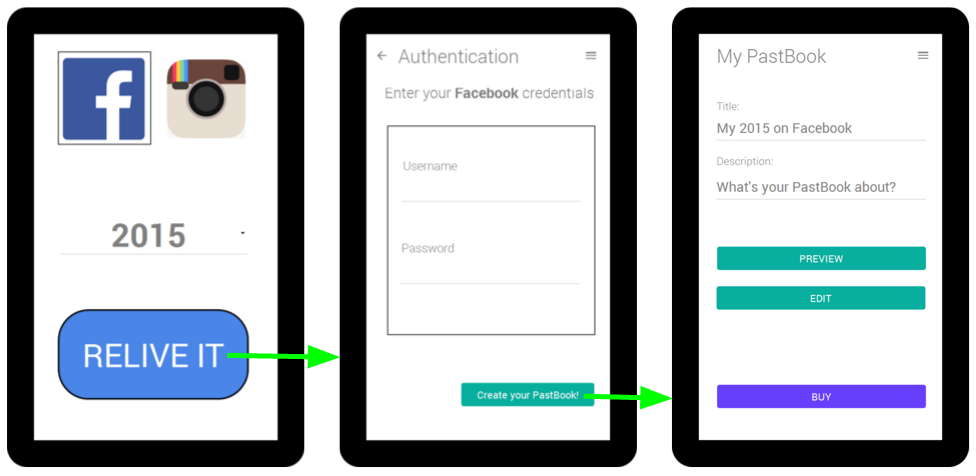
\includegraphics[width=0.9\textwidth]{capitolo_3/immagini/wireframe_1.png}
					\caption{Rappresentazione del processo di creazione di un Photo Book nell'applicazione.}
				\end{figure}
				\noindent L'utente ha la possibilità di scegliere il social network dal quale ottenere le immagini (nello specifico
				Facebook o Instagram). Egli, inoltre, può scegliere l'anno durante il quale sono state scattate le foto che desidera
				inserire all'interno del Photo Book. Può infine cliccare sul pulsante \emph{Relive it}. A questo punto all'utente
				sono richieste le credenziali per accedere al social network scelto e procedere con l'autorizzazione. Dopo che
				l'autenticazione è andata a buon fine e i permessi sono stati concessi viene creato il Photo Book. L'utente entra
				in una scehrmata di riepilogo, dove ha tre opzioni: visualizzare l'album, modificarlo o procedere con il pagamento.
				\begin{figure}[H]
					\centering
					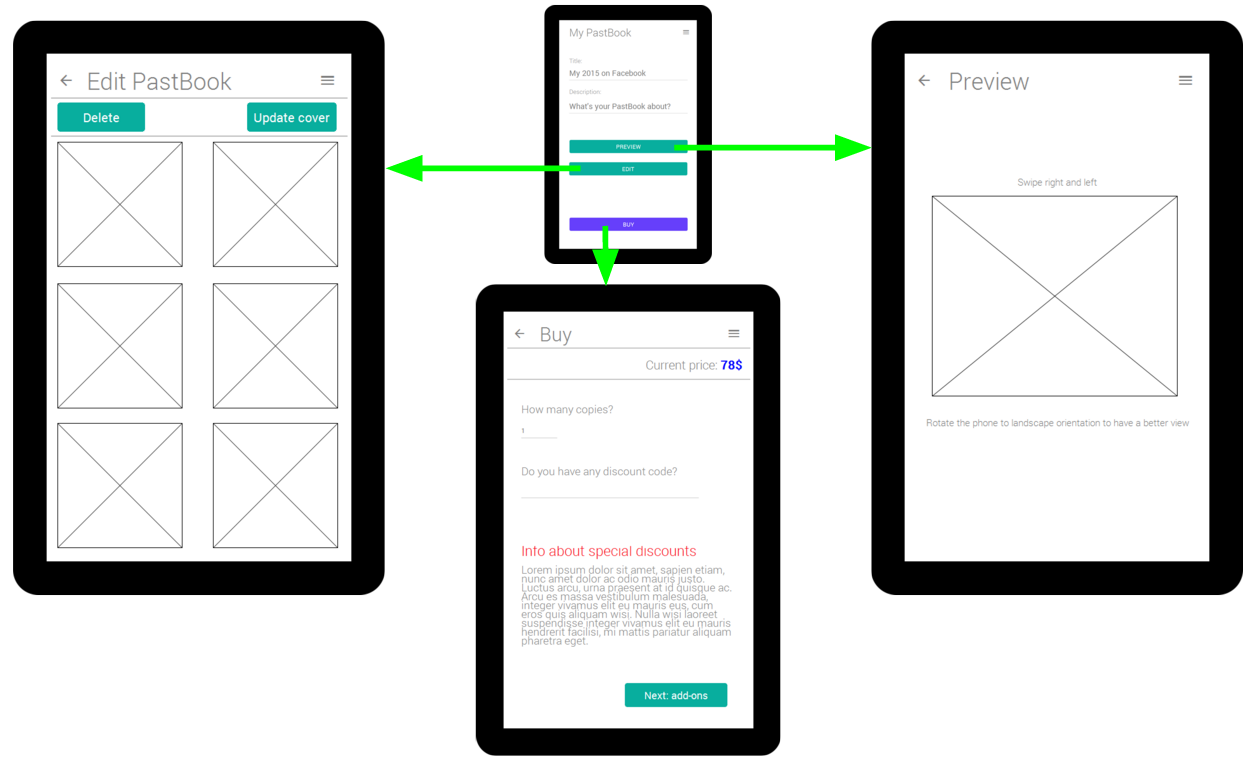
\includegraphics[width=0.9\textwidth]{capitolo_3/immagini/wireframe_2.png}
					\caption{Rappresentazione delle opzioni che l'utente ha dopo la creazione del Photo Book.}
				\end{figure}
				\noindent La schermata dedicata alle modifiche permette di selezionare le immagini presenti nel Photo Book per poter
				scegliere la nuova copertina o per cancellare foto indesiderate. La schermata dedicata alla visualizzazione
				dell'album permette di sfogliare virtualmente il Photo Book.
				\begin{figure}[H]
					\centering
					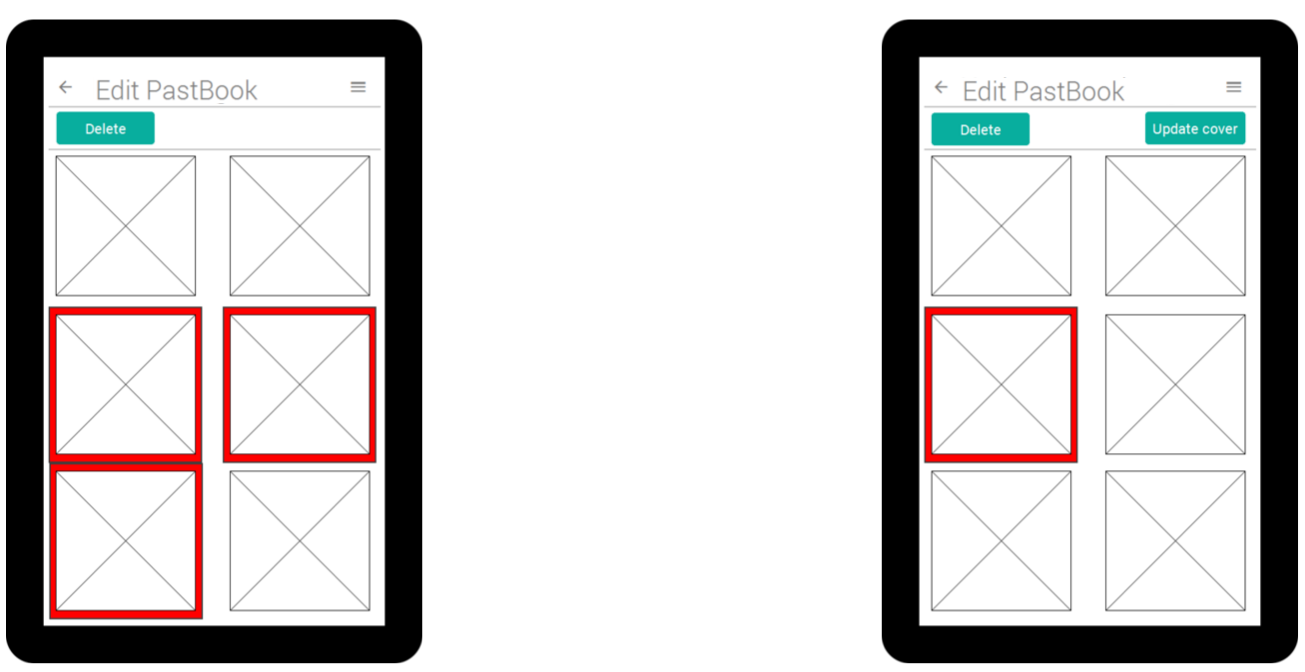
\includegraphics[width=0.9\textwidth]{capitolo_3/immagini/wireframe_3.png}
					\caption{Rappresentazione delle opzioni che l'utente ha per modificare il Photo Book.}
				\end{figure}
				\noindent La schermata delle modifiche, in particolare, permette all'utente di selezionare una o più immagini. Se le
				immagini selezionate sono più di una allora è utilizzabile solo il pulsante adibito alla cancellazione delle foto.
				Se la selezione comprende una singola immagine allora l'utente può scegliere se eliminarla o utilizzarla per
				sostituire la vecchia copertina del Photo Book.
				\begin{figure}[H]
					\centering
					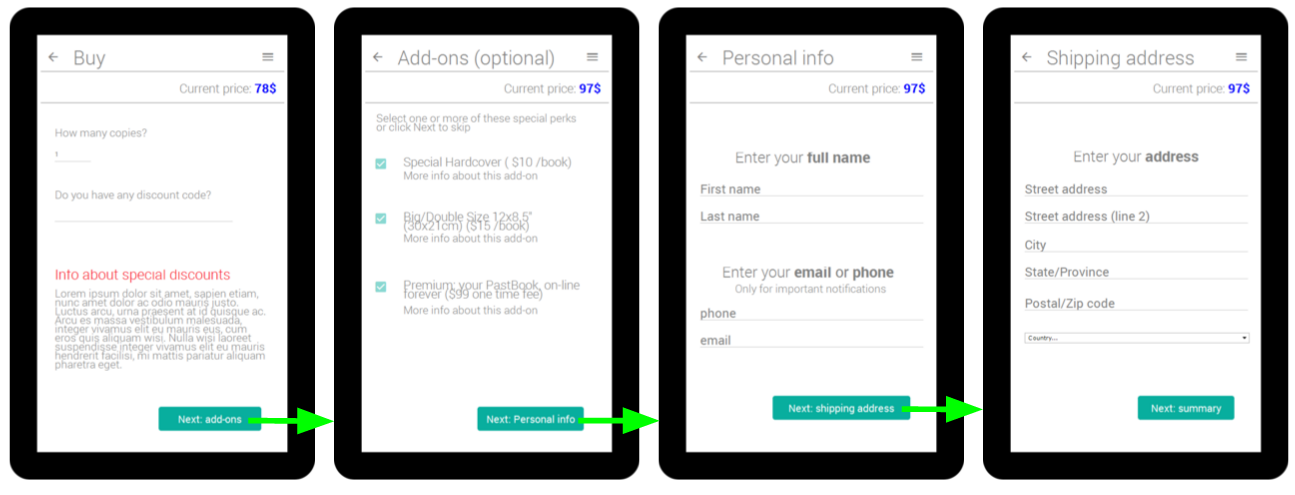
\includegraphics[width=0.9\textwidth]{capitolo_3/immagini/wireframe_4.png}
					\caption{Rappresentazione dei passaggi necessari per effettuare il pagamento.}
				\end{figure}
				\noindent Il pagamento del Photo Book è realizzato utilizzando più schermate. Nella prima l'utente indica il numero
				di copie desiderate e se è in possesso di speciali codici per sconti aggiuntivi. Nella seconda schermata l'utente può
				scegliere se aggiungere alcuni pacchetti opzionali (per esempio copertine rigide o album più grandi). Procedendo egli
				fornisce a PastBook i dettagli personali e i metodi tramite il quale preferisce essere contattato. Infine, compila
				i dati riguardanti l'indirizzo al quale intende ricevere il prodotto una volta che è stato stampato con successo.\\
				In seguto alla presentazione ho discusso con il mio tutor su quali fossero effettivamente le funzionalità che avrei
				dovuto implementare e come sarebbe dovuta essere strutturata l'applicazione: i cambiamenti più significativi
				rispetto a ciò che avevo pensato e sui quali abbiamo concordato riguardano i seguenti aspetti:
				\begin{itemize}
					\item Deve essere implementato una schermata di attesa e/o intrattenimento subito dopo l'autenticazione da
					parte dell'utente. Questo è necessario a causa della lunghezza del processo di realizzazione del Photo Book.
					\item Non appena il processo di realizzazione del Photo Book è stato concluso l'utente deve poter
					visualizzare immediatamente l'album prodotto, senza dover cliccare su un ulteriore pulsante. I pulsanti di
					modifica e pagamento devono essere all'interno della stessa schermata.
				\end{itemize}
			\subsubsection{Design e marketing}
				Descrivo come una parte fondamentale dell'analisi dei requisiti (svolta verso la fine dello stage) abbia riguardato
				il design che l'applicazione avrebbe dovuto avere. Descrivo come ho collaborato con un esperto per poter capire
				cosa fosse possibile e sensato aggiungere. Descrivo inoltre come durante l'analisi molti dei particolari aggiunti
				riguardassero puro marketing, e come abbia dovuto scendere a compromessi con principi di usabilità e accessibilità.
				Descrivo come si desiderasse che l'utente non si accorgesse dei tempi di attesa (quindi lo si voleva distrarre) e
				allo stesso tempo arrivasse con un singolo click alla creazione e visualizzazione del photo book, in linea con
				gli obiettivi aziendali. Descrivo tutte le opzioni che sono state considerate a tal proposito.
		\subsection{Progettazione}
			\subsubsection{Modularizzazione della struttura dell'applicazione}
				Descrivo come si è svolta l'attività di progettazione e in particolare riporto alcuni dei risultati. Descrivo come
				l'applicazione sia stata suddivisa in moduli riutilizzabili in più schermate e anche in applicazioni simili. 
				Descrivo come siano stati sfruttati alcuni pattern per semplificare la struttura, la comprensibilità e l'utilizzo
				delle varie classi.
			\subsubsection{Utilizzo delle funzioni di PastBook Mobile SDK}
				Descrivo come l'applicazione sia pensata per far pesante uso delle funzioni messe a disposizione dall'SDK creato in
				precedenza. Descrivo come l'SDK eviti molto lavoro a chi deve sviluppare una nuova applicazione per l'azienda.
		\subsection{Implementazione delle schermate e dei relativi controller}
			\subsubsection{L'uso del framework MVC Alloy}
				Descrivo come ho utilizzato il framework ALloy (messo a disposizione da Appcelerator) per implementare in modo
				facile il pattern MVC. Descrivo i vantaggi derivanti dall'utilizzo di tale framework rispetto all'uso della versione
				base di Titanium. Descrivo le motivazioni della mia scelta.
			\subsubsection{Creazione di un Photo Book}
				Descrivo la schermata iniziale dell'applicazione. Descrivo come essa è stata implementata e quali sono i principali
				elementi presenti in essa. Descrivo come molti di essi siano riutilizzabili altrove (in altre schermate o anche
				altre applicazioni). Descrivo le principali animazioni che sono state implementate in seguito all'analisi dei
				requisiti dedicata.
			\subsubsection{Intrattenimento dell'utente}
				Descrivo la schermata dedicata all'intrattenimento dell'utente durante la creazione di un photo book. Descrivo come
				le finalità di tale schermata avessero scopi di puro marketing (si vuole distrarre l'utente durante l'attesa).
				Descrivo come l'impossibilità di implementare alcuni particolari (a causa di bug del framework) abbiano comportato
				dei cambiamenti nell'analisi dei requisiti. Descrivo il risultato al quale si è arrivati alla fine. Descrivo i
				problemi che esso ha causato sia in termini di prestazioni su dispositivi lenti che in termini di memoria utilizzata.
				Descrivo come tale schermata sia stata ottimizzata.
			\subsubsection{Visualizzazione del Photo Book}
				Descrivo la schermata dedicata alla visualizzazione del photo book. Descrivo come sia stato implementato il libro
				3d sfogliabile dall'utente. Descrivo i problemi che l'implementazione di tale schermata ha comportato (dovuti
				soprattutto all'orientamento del telefono). Descrivo come tali problemi sono stati affrontati e risolti. Descrivo
				infine la possibilità per l'utente di condividere il photo book creato e di votare l'applicazione sullo store
				(solo in determinate situazioni, ovvero quando si presume che all'utente l'applicazione sia piaciuta).
			\subsubsection{Modifica del Photo Book}
				Descrivo le schermate grazie alle quali un utente può modificare i propri photo book. Descrivo come la sua
				implementazione sia stata semplice grazie all'uso dell'SDK. Descrivo come gestisce e corregge eventuali errori senza
				che l'utente se ne accorga. Descrivo come sia stato possibile riutilizzare molti degli elementi presenti nella
				schermata di intrattenimento.
			\subsubsection{Checkout}
				Descrivo la schermata nella quale l'utente può comprare il photo book creato. Descrivo perchè ho deciso assieme
				all'azienda di implementarla facendo largo uso di una webview invece che di elementi nativi.
		\subsection{Verifica dei risultati ottenuti}
			Descrivo come sia stata effettuata l'attività di verifica sull'applicazione. Spiego che la parte principale è stata
			svolta mediante l'utilizzo di emulatori e grazie a una serie di test decisi a priori e documentati (seppur non
			automatizzati). Spiego inoltre come consegnassi quasi giornalmente un prototipo a 5-6 persone che si preoccupavano
			di provare l'applicazione e di segnalare malfunzionamenti o rallentamenti. Spiego come ho implementato un sistema
			che permetteva ai tester di essere più precisi possibile riguardo gli errori che erano riportati.
	\section{Mantenimento di My Year Photo Book}
		\subsection{Rilascio dell'applicazione}
			Descrivo in che modo l'applicazione è stata resa disponibile al pubblico per il beta testing. Descrivo gli strumenti
			utilizzati e gli utenti ai quali è stato dato l'accesso alla preview.
		\subsection{Raccolta dei dati}
			Descrivo in che modo e con quali tecnologie si sono raccolti i dati di utilizzo da parte degli utenti e i dati riguardanti
			eventuali crash dell'applicazione. Descrivo in base a quali principi si è scelto di raccogliere certi dati piuttsto che altri
		\subsection{Analisi dei dati}
			Descrivo in che modo ho proceduto all'analisi dei dati provenienti dagli utenti che stavano utilizzando l'applicazione in
			anteprima. Descrivo come grazie ai dati e ai feedback ho potuto trovare e correggere alcuni errori. Descrivo a quali
			conclusioni sono arrivato studiando i dati di utilizzo a disposizione e come ho proposto all'azienda quali sarebbero stati
			gli aspetti migliorabili da un punto di vista della soddisfazione degli utenti
	\section{Analisi dei principali problemi}
		\subsection{Criticità riscontrate usando Titanium}
			\subsubsection{Documentazione scadente e community limitata}
				Ho dovuto scontrarmi con molti limiti di Titanium durante l'intera esperienza di Stage. Il problema più serio
				riguarda probabilmente gli strumenti a supporto degli sviluppatori: la documentazione ufficiale e la community di
				utilizzatori dei prodotti Appcelerator.\\
				In primo luogo, la documentazione ufficiale alla quale facevo riferimento si è rivelata essere spesso inappropriata e
				di qualità scadente. In particolare, i problemi riscontrati sono stati:
				\begin{itemize}
					\item \emph{Organizzazione confusa}, in quanto spesso risultava complicato cercare le descrizioni delle API
					necessarie ad alcuni scopi. La confusione generale poteva essere anche notata dal fatto che molti link non
					erano stati aggiornati correttamente e conducevano quindi a sezioni con contenuti obsoleti.
					\item \emph{Presenza di alcuni errori}, in quanto mi è capitato di trovare delle API che svolgevano le
					operazioni in modo differente rispetto a quanto descritto nella documentazione. In questi casi ho avuto
					l'accortezza di segnalare la cosa ad Appcelerator.
				\end{itemize}
				Ritengo che la documentazione sia uno strumento fondamentale per gli sviluppatori, oltre che l'immagine della serietà
				dell'azienda. Dal mio punto di vista, dunque, è impensabile che essa presenti questi problemi.\\
				Un secondo punto a svantaggio degli utilizzatori di Titanium è la community di Appcelerator. Essa è per forza di cose
				molto più contenuta rispetto a quelle degli sviluppatori Android o iOS. Ne consegue un dettaglio non trascurabile per
				coloro che si approcciano per la prima volta a questa piattaforma: spesso non esiste una soluzione ai propri problemi
				che sia rintracciabile in rete. La maggior parte delle volte ognuno è tenuto ad esplorare personalmente gli strumenti
				per cercare di individuare delle spiegazioni plausibili.
			\subsubsection{Sviluppo cross-platform impossibile}
				Titanium è un prodotto pensato per realizzare applicazioni cross-platform native. Tuttavia, esso non riesce
				completamente nel suo scopo. Infatti, vi sono ovviamente delle funzionalità che sono disponibili su iOS ma non su
				Android, e viceversa. Appcelerator non tenta di uniformare le differenze ma permette semplicemente l'esecuzione di
				alcune API solo su determinate piattaforme mobile. Ne consegue che il programmatore deve:
				\begin{itemize}
					\item controllare continuamente la compatibilità delle API utilizzate;
					\item utilizzare le API non compatibili con altre piattaforme all'interno di istruzioni condizionali;
					\item prevedere alternative per le varie piattaforme.
				\end{itemize}
				L'ultimo punto, in particolare, risulta particolarmente critico. Infatti, talvolta può accadere che iOS e Android
				gestiscano situazioni simili in modo completamente diverso, se non opposto. Questo comporta che lo sviluppatore deve
				prevedere modalità di funzionamento completamente diverse all'interno dello stesso codice, complicando non poco il
				software prodotto.\\
				Da questo punto di vista, i maggiori problemi pratici con cui mi sono scontrato sono:
				\begin{itemize}
					\item Gestione degli elementi — e in particolare delle finestre — trasparenti. In un caso essi permettono
					agli elementi sottostanti di essere cliccabili, nell'altro si comportano in modo opposto.
					\item Gestione della disabilitazione dello zoom nelle webview. In un caso si nascondono solo i tasti virtuali
					presenti sullo schermo, nell'altro si disabilita anche il \emph{pinch to zoom} e il \emph{double tap}.
				\end{itemize}
				Infine, come se non bastasse, Titanium non si occupa nemmeno del fatto che versioni differenti della stessa
				piattaforma richiedano API diverse. Ne consegue che lo sviluppatore deve controllare continuamente anche 
				la compatibilità delle varie API con versioni diverse di una stessa piattaforma.\\
				Quando ci si è concentrati sull'aspetto grafico	dell'applicazione le difficoltà sono risultate essere eccessive: a
				testimonianza di questo fatto ho preso la decisione di suddividere lo sviluppo dell'applicazione Android da quello
				della versione per iOS in comune accordo con il tutor e il dirigente aziendale.\\
				È mio parere personale che l'uso di Titanium a queste condizioni non abbia molto senso: infatti, esso è un prodotto
				pensato per lo sviluppo cross-platform e dunque dovrebbe giungere ad alcuni compromessi pur di offrire davvero
				la possibilità di scrivere un codice unico per creare più versioni della stessa applicazione.
			\subsubsection{Presenza di bug}
				Un'ultima criticità incontrata nell'utilizzo di Titanium riguarda la presenza di alcuni bug all'interno di certe API.
				\begin{itemize}
					\item Il ridimensionamento delle immagini non viene fatto in modo corretto. Il comando in questione, nel
					dettaglio, non riesce a riconoscere l'altezza e la larghezza reali dei file: ne deriva un'immagine
					inutilizzabile nella quale la proporzione delle dimensioni non è stata rispettata.
					\item Il modulo per l'autenticazione e l'autorizzazione tramite Facebook non funziona in modo corretto su
					Android. Nel dettaglio, esso non genera tutti gli eventi descritti nella documentazione.
				\end{itemize}
		\subsection{Difficoltà dovute al metodo di lavoro utilizzato}
			\subsubsection{Rallentamenti causati dalla necessità di numerosi prototipi}
				Il metodo di lavoro al quale ho dovuto adattarmi in azienda imponeva che consegnassi continuamente dei prototipi
				funzionanti di My Year Photo Book. Durante alcuni periodi della mia esperienza di stage dovevo consegnare anche una
				versione al giorno dell'applicazione.\\
				Questo modo di procedere da un lato mi ha dato la possibilità di far testare il mio prodotto ad altre persone,
				dall'altro mi ha rallentato notevolmente durante lo sviluppo. Infatti, quando dovevo consegnare un prototipo dovevo
				lasciare da parte le sperimentazioni che stavo portando avanti per dare priorità alla correzione di eventuali errori
				e alla configurazione di un eseguibile che fosse installabile su un dispositivo reale invece che su un emulatore. Ne
				conseguiva che per una discreta parte della mia giornata lavorativa non potessi progredire nello sviluppo di nuove
				funzionalità del prodotto.\\
				Dal mio punto di vista sarebbe stato più utile diminuire la frequenza delle consegne per permettere una miglior
				organizzazione del tempo da parte dello sviluppatore.
			\subsubsection{Modifiche all'architettura software}
				Non è stato dedicato tempo a una vera e propria attività di progettazione architetturale durante la quale fosse
				possibile definire la struttura del software. Ho piuttosto proceduto seguendo le indicazioni dell'azienda e del mio
				tutor, che mi hanno incitato a consegnare nel giro di pochi giorni un prodotto funzionante con caratteristiche
				minimali.\\
				L'enorme difetto di questo modo di procedere consisteva nel fatto che ero completamente alle prime armi
				nell'utilizzare Titanium e dunque non sapevo quali fossero le migliori strategie e pattern da adottare: il risultato
				è stato che l'architettura da me adottata inizialmente non era facilmente manutenibile, seppur funzionante. Il
				problema si è rivelato essere più grave del previsto quando le dimensioni dell'applicazione hanno cominciato
				a crescere: l'intera struttura del software non risultava più utilizzabile. Dopo essersi accorto di questo, il
				dirigente aziendale mi ha prima concesso del tempo per pensare a una possibile riorganizzazione del lavoro da me
				svolto e in seguito mi ha affiancato qualcuno che mi aiutasse a convertire tutto il lavoro fatto nel mese precedente
				alla nuova architettura. Questa attività ha rallentato lo sviluppo dell'applicazione di almeno 3-4 giorni.\\
				In seguito a questa esperienza l'azienda ha deciso di investire una quota maggiore del mio tempo sull'analisi del
				problema, riducendo al contempo la frequenza con la quale ero tenuto a consegnare i prototipi del prodotto.
